% ========================
% estilo.latex mínimo funcional
% ========================

\documentclass[12pt]{book} % report para capítulos

% ========================
% Paquetes y comandos extra
% ========================
% ===========================
% Paquetes básicos de idioma y codificación
% ===========================
\usepackage[utf8]{inputenc}   % Codificación UTF-8
\usepackage[T1]{fontenc}      % Acentos y caracteres correctos
\usepackage[spanish]{babel}   % Traducción al español (capítulos, índices, etc.)
\usepackage{csquotes}         % Citas tipográficas correctas

% ===========================
% Tipografía
% ===========================
\usepackage{lmodern}          % Fuente Latin Modern
\usepackage{microtype}        % Mejoras tipográficas (espaciado, justificación)

% ===========================
% Márgenes y geometría
% ===========================
\usepackage{geometry}         % Control de márgenes
\geometry{a4paper, top=3cm, bottom=3cm, left=3cm, right=3cm}

% ===========================
% Matemáticas
% ===========================
\usepackage{amsmath, amssymb, amsthm} % Paquetes AMS
\usepackage{mathtools}        % Extiende amsmath
\usepackage{physics}          % Notación física y matemática (derivadas, bra-ket, etc.)
\usepackage{siunitx}          % Unidades SI (e.g. \SI{3}{m/s})
% \sisetup{locale=ES}           % Configuración para español (coma decimal, etc.)
\AtBeginDocument{\RenewCommandCopy\qty\SI} % Resolve siunitx and physics conflict


% ===========================
% Gráficos, tablas y colores
% ===========================
\usepackage{graphicx}         % Insertar imágenes
\usepackage{xcolor}           % Colores personalizados
\usepackage{tikz}             % Dibujos vectoriales
\usetikzlibrary{calc,positioning,shapes,arrows} % Librerías útiles de TikZ
\usepackage{pgfplots}         % Gráficas de funciones
\pgfplotsset{compat=1.18}
\usepackage{float}            % Control de posición de figuras/tablas
\usepackage{booktabs}         % Tablas profesionales
\usepackage{multirow}         % Celdas que ocupan varias filas
\usepackage{array}            % Más control en tablas
\usepackage{colortbl}         % Tablas con colores
\usepackage{inconsolata}


% ===========================
% Listas y enumeraciones
% ===========================
\usepackage{enumitem}         % Control de listas enumeradas y viñetas

% ===========================
% Encabezados, pies y diseño
% ===========================
\usepackage{fancyhdr}         % Encabezados y pies de página
\usepackage{titlesec}         % Personalizar títulos de capítulos/secciones
\usepackage{setspace}         % Espaciado entre líneas
\usepackage{parskip}          % Control del espacio entre párrafos

% ===========================
% Referencias, hipervínculos y citas
% ===========================
\usepackage{hyperref}         % Hipervínculos en PDF
\hypersetup{
    colorlinks = true,
    linkcolor  = red!70,
    citecolor  = red!70,
    urlcolor   = red!70,
    pdfpagelayout = SinglePage, % Asegura que el contenido se ajuste a una sola página
    pdfstartview = Fit          % Ajusta el contenido al tamaño de la página
}
\usepackage{cleveref}         % Referencias inteligentes (\cref)

% ===========================
% Código fuente
% ===========================
\usepackage{listings}         % Mostrar código con estilo
\usepackage{minted}           % (mejor opción, requiere Python y pygments)

% ===========================
% Bibliografía
% ===========================
\usepackage[backend=biber,style=apa]{biblatex} % Ejemplo: estilo APA
\addbibresource{referencias.bib}              % Archivo .bib

% ===========================
% Otros útiles
% ===========================
\usepackage{pdfpages}         % Insertar PDFs externos
\usepackage{blindtext}        % Texto de prueba
\usepackage{caption}          % Personalizar pies de figura/tabla
\usepackage{subcaption}       % Subfiguras
\usepackage{tocloft} 
\usepackage{amsthm}
\usepackage{subcaption}
\usepackage{truncate} % permite truncar texto si no cabe
\usepackage{libertinus}  % reemplaza lmodern
\usepackage{booktabs}  % para \toprule, \midrule, \bottomrule
\usepackage{array}     % para definir columnas personalizadas
\usepackage{colortbl}  % colores en tablas
\usepackage{etoolbox}
\AtBeginEnvironment{tabular}{\rowcolors{2}{gray!10}{white}\renewcommand{\arraystretch}{1.2}}

% ===========================
% Opciones de fuentes sugeridas
% ===========================
% TeX Gyre Pagella (estilo Palatino)
% \usepackage{fontspec}
% \usepackage{unicode-math}
% \setmainfont{TeX Gyre Pagella}
% \setmathfont{TeX Gyre Pagella Math}

% TeX Gyre Termes (estilo Times)
% \setmainfont{TeX Gyre Termes}
% \setmathfont{TeX Gyre Termes Math}

% Libertinus (elegante y completa)
% \setmainfont{Libertinus Serif}
% \setmathfont{Libertinus Math}

% TeX Gyre Bonum (estilo Garamond)
% \setmainfont{TeX Gyre Bonum}
% \setmathfont{TeX Gyre Bonum Math}

% Latin Modern (moderno de Computer Modern)
% \setmainfont{Latin Modern Roman}
% \setmathfont{Latin Modern Math}


% \usepackage{helvet}
% \usepackage{libertine}
% \usepackage[sfdefault]{FiraSans}

\usepackage{tcolorbox} % para cajas de colores




  % si tienes paquetes personalizados
% aquí van los comandos personalizados
% Comando para incluir imágenes
\newcommand{\incluirimagen}[3][]{%
\begin{figure}[H]
    \centering
    \includegraphics[width=\linewidth,#1]{#2}
    \caption{#3}
    \label{fig:#2}
\end{figure}
}

% comando para ejercicios con fondo
\newtheoremstyle{ejerciciostyle}
  {10pt}   % Espacio arriba
  {10pt}   % Espacio abajo
  {\itshape} % Fuente del cuerpo
  {}       % Sangría
  {\bfseries} % Fuente del encabezado
  {}      % Puntuación tras encabezado
  { }      % Espacio tras encabezado
  {\thmname{#1} \thmnumber{#2}. \thmnote{#3}}


% % comando formal para enunciado de ejercicios
% \theoremstyle{ejerciciostyle}
% \newtheorem{ejercicio}{Ejercicio}[chapter]

\theoremstyle{ejerciciostyle}
\newtheorem{ejercicio}{Ejercicio}[section]

\renewcommand{\theejercicio}{\thechapter.\arabic{section}.\arabic{ejercicio}}


% comando formal para soluciones
\theoremstyle{remark}
\newtheorem*{solucion}{Solución}

% Comando para dos imágenes en paralelo
\newcommand{\dosimagenes}[6]{%
    \begin{figure}[h!]
        \centering
        \begin{minipage}{0.48\linewidth}
            \centering
            \includegraphics[width=\linewidth]{#1}
            \caption{#2}
            \label{#5}
        \end{minipage}\hfill
        \begin{minipage}{0.48\linewidth}
            \centering
            \includegraphics[width=\linewidth]{#3}
            \caption{#4}
            \label{#6}
        \end{minipage}
    \end{figure}
}

% \dosimagenes{media/fondo.jpg}{Descripción 1}{media/fondo.jpg}{Descripción 2}{fig:descripcion1}{fig:descripcion2}

% \ref{fig:descripcion1} es la mejor
% \ref{fig:descripcion2} es la mejor

\newcommand{\portadaimg}{\VAR{portadaimg}}

% Comando para crear una nota estilo información
\newcommand{\nota}[2]{%
\begin{tcolorbox}[colframe=blue!75!black, colback=blue!5!white, title=\textbf{#1}]
    #2
\end{tcolorbox}
}
  % comandos LaTeX propios
% ===========================
% Diseño general
% ===========================
\setstretch{1.15} % interlineado
\setlength{\parskip}{0.5em} % espacio entre párrafos
\setlength{\parindent}{0pt} % sin sangría

% ===========================
% Estilo de capítulos y secciones (titlesec)
% ===========================
\titleformat{\chapter}[display]
  {\bfseries\Huge}
  {\filleft\Large\scshape Capítulo \thechapter}
  {1ex}
  {\titlerule[1pt]\vspace{1ex}\filright}
  [\vspace{1ex}\titlerule]

\titlespacing*{\chapter}{0pt}{0pt}{2em}

\titleformat{\section}
  {\Large\bfseries}
  {\thesection}{1em}{}

\titleformat{\subsection}
  {\large\bfseries}
  {\thesubsection}{1em}{}

\titleformat{\subsubsection}
  {\normalsize\bfseries\itshape}
  {\thesubsubsection}{1em}{}

% ===========================
% Encabezados y pies de página (fancyhdr)
% ===========================
\pagestyle{fancy}
\fancyhf{} % limpia
\fancyhead[L]{\small\scshape\nouppercase{\leftmark}} % sección/capítulo en mayúsculas pequeñas
\fancyhead[R]{\small\thepage}                        % número de página
%\fancyfoot[C]{\scriptsize\itshape Apuntes de la carrera} % texto fijo abajo en cursiva
% Encabezados y pies de página personalizados
% \fancyfoot[L]{\scriptsize\itshape Nombre de la asignatura} % pie de página izquierdo en cursiva
\fancyfoot[R]{\scriptsize\itshape Ismael Sallami Moreno}        % pie de página derecho con el nombre del autor

% Línea bajo el encabezado
\renewcommand{\headrulewidth}{0.5pt} % línea más gruesa en el encabezado
% Línea en el pie
\renewcommand{\footrulewidth}{0.4pt} % línea fina en el pie
\renewcommand{\sectionmark}[1]{%
  \markboth{\thesection\quad #1}{}%
}

% ===========================
% Numeración de elementos
% ===========================
\numberwithin{equation}{chapter} % ecuaciones numeradas por capítulo
\numberwithin{figure}{chapter}   % figuras numeradas por capítulo
\numberwithin{table}{chapter}    % tablas numeradas por capítulo

% ===========================
% Listas y enumeraciones
% ===========================
\setlist[itemize]{label=--, left=1.5em}
\setlist[enumerate]{label=\arabic*), left=1.5em}

% ===========================
% Estilo de citas y bibliografía
% ===========================
\DefineBibliographyStrings{spanish}{%
  references = {Bibliografía},
}

% ===========================
% Entornos personalizados
% ===========================
\newtheoremstyle{cajita} % nombre del estilo
  {1em}   % espacio arriba
  {1em}   % espacio abajo
  {}      % fuente del cuerpo
  {}      % indentación
  {\bfseries} % fuente del título
  {.}     % puntuación tras título
  {0.5em} % espacio tras título
  {\thmname{#1}\thmnumber{ #2} \thmnote{(#3)}} % formato

\theoremstyle{cajita}
\newtheorem{teorema}{Teorema}[chapter]
\newtheorem{definicion}{Definición}[chapter]
\newtheorem{ejemplo}{Ejemplo}[chapter]
\newtheorem{proposicion}{Proposición}[chapter]

% ===========================
% Configuración de lstlisting
% ===========================

% ===============================================
% ESTILO 1: MODERNO Y MINIMALISTA
% ===============================================

% Definir colores personalizados
\definecolor{codegreen}{rgb}{0,0.6,0}
\definecolor{codegray}{rgb}{0.5,0.5,0.5}
\definecolor{codepurple}{rgb}{0.58,0,0.82}
\definecolor{backcolour}{rgb}{0.95,0.95,0.92}
\definecolor{framecolor}{rgb}{0.8,0.8,0.8}

\lstset{
    backgroundcolor=\color{backcolour},   
    commentstyle=\color{codegreen},
    keywordstyle=\color{magenta},
    numberstyle=\tiny\color{codegray},
    stringstyle=\color{codepurple},
    basicstyle=\ttfamily\footnotesize,
    breakatwhitespace=false,         
    breaklines=true,                 
    captionpos=b,                    
    keepspaces=true,                 
    numbers=left,                    
    numbersep=5pt,                  
    showspaces=false,                
    showstringspaces=false,
    showtabs=false,                  
    tabsize=2,
    frame=shadowbox,
    frameround=tttt,
    rulecolor=\color{framecolor},
    rulesepcolor=\color{framecolor},
    xleftmargin=20pt,
    xrightmargin=20pt,
    aboveskip=20pt,
    belowskip=20pt
}

% ===============================================
% ESTILO 2: ELEGANTE CON BORDES REDONDEADOS
% ===============================================

% Colores para estilo elegante
\definecolor{lightblue}{rgb}{0.93,0.95,1}
\definecolor{darkblue}{rgb}{0.1,0.2,0.5}
\definecolor{mediumblue}{rgb}{0.2,0.4,0.8}
\definecolor{darkgreen}{rgb}{0,0.5,0}
\definecolor{darkred}{rgb}{0.6,0,0}

\lstdefinestyle{elegant}{
    backgroundcolor=\color{lightblue},
    commentstyle=\color{darkgreen}\itshape,
    keywordstyle=\color{darkblue}\bfseries,
    numberstyle=\tiny\color{gray},
    stringstyle=\color{darkred},
    basicstyle=\ttfamily\small,
    breakatwhitespace=false,
    breaklines=true,
    captionpos=t,
    keepspaces=true,
    numbers=left,
    numbersep=8pt,
    showspaces=false,
    showstringspaces=false,
    showtabs=false,
    tabsize=4,
    frame=single,
    frameround=tttt,
    framesep=10pt,
    xleftmargin=15pt,
    xrightmargin=15pt,
    aboveskip=15pt,
    belowskip=15pt,
    columns=flexible
}

% ===============================================
% ESTILO 3: PROFESIONAL CORPORATIVO
% ===============================================

% Colores corporativos
\definecolor{corporatebg}{rgb}{0.98,0.98,0.98}
\definecolor{corporateblue}{rgb}{0.07,0.29,0.49}
\definecolor{corporategray}{rgb}{0.4,0.4,0.4}
\definecolor{corporategreen}{rgb}{0.13,0.55,0.13}
\definecolor{corporatered}{rgb}{0.8,0.2,0.2}

\lstdefinestyle{corporate}{
    backgroundcolor=\color{corporatebg},
    commentstyle=\color{corporategreen}\slshape,
    keywordstyle=\color{corporateblue}\bfseries,
    numberstyle=\scriptsize\color{corporategray},
    stringstyle=\color{corporatered},
    basicstyle=\ttfamily\footnotesize,
    breakatwhitespace=false,
    breaklines=true,
    captionpos=b,
    keepspaces=true,
    numbers=left,
    numbersep=12pt,
    showspaces=false,
    showstringspaces=false,
    showtabs=false,
    tabsize=3,
    frame=leftline,
    framerule=3pt,
    rulecolor=\color{corporateblue},
    xleftmargin=25pt,
    aboveskip=20pt,
    belowskip=20pt,
    lineskip=1pt
}

% ===============================================
% ESTILO 4: MODERNO CON SOMBRAS
% ===============================================

% Colores modernos
\definecolor{modernbg}{rgb}{0.97,0.97,0.97}
\definecolor{moderngray}{rgb}{0.3,0.3,0.3}
\definecolor{modernpurple}{rgb}{0.5,0.2,0.8}
\definecolor{modernteal}{rgb}{0,0.5,0.5}
\definecolor{modernorange}{rgb}{0.8,0.4,0}

\lstdefinestyle{modern}{
    backgroundcolor=\color{modernbg},
    commentstyle=\color{modernteal}\itshape,
    keywordstyle=\color{modernpurple}\bfseries,
    numberstyle=\tiny\color{moderngray},
    stringstyle=\color{modernorange},
    basicstyle=\ttfamily\small,
    breakatwhitespace=false,
    breaklines=true,
    captionpos=t,
    keepspaces=true,
    numbers=left,
    numbersep=10pt,
    showspaces=false,
    showstringspaces=false,
    showtabs=false,
    tabsize=4,
    frame=tb,
    framerule=2pt,
    rulecolor=\color{modernpurple},
    xleftmargin=20pt,
    xrightmargin=20pt,
    aboveskip=25pt,
    belowskip=25pt
}

% ===============================================
% CONFIGURACIÓN PARA DIFERENTES LENGUAJES
% ===============================================

% Python
\lstdefinestyle{python}{
    language=Python,
    style=elegant,
    morekeywords={True,False,None,self,cls,def,class,import,from,as,with,yield,async,await},
    morecomment=[l]{\#},
    morestring=[b]',
    morestring=[b]"
}

% Java
\lstdefinestyle{java}{
    language=Java,
    style=corporate,
    morekeywords={var,record,sealed,permits,non-sealed}
}

% C++
\lstdefinestyle{cpp}{
    language=C++,
    style=modern,
    morekeywords={constexpr,nullptr,auto,decltype,override,final}
}

% JavaScript
\lstdefinestyle{javascript}{
    language=Java,
    style=elegant,
    morekeywords={let,const,var,function,class,extends,import,export,default,async,await,yield},
    morecomment=[l]{//},
    morecomment=[s]{/*}{*/},
    morestring=[b]',
    morestring=[b]",
    morestring=[b]`
}

% ===============================================
% EJEMPLOS DE USO
% ===============================================

% Para usar el estilo por defecto:
% \begin{lstlisting}
% código aquí
% \end{lstlisting}

% Para usar un estilo específico:
% \begin{lstlisting}[style=elegant]
% código aquí
% \end{lstlisting}

% Para incluir un archivo con estilo específico:
% \lstinputlisting[style=python]{archivo.py}

% Para código inline:
% \lstinline[style=modern]{código inline}

% ===============================================
% CONFIGURACIÓN ADICIONAL PARA TÍTULOS Y CARACTERES
% ===============================================

% Personalizar el formato de los títulos de los listados
\renewcommand\lstlistingname{Código}
\renewcommand\lstlistlistingname{Lista de Códigos}

% Configurar el formato del título con soporte para tildes
\lstset{
    title=\lstname,
    captionpos=t,
    abovecaptionskip=10pt,
    belowcaptionskip=5pt,
    % Configuración global para caracteres especiales
    inputencoding=utf8,
    extendedchars=true
}

% ===============================================
% COMANDOS PERSONALIZADOS ÚTILES
% ===============================================

% Comando para código inline con soporte automático de tildes
\newcommand{\codeinline}[2][modern]{\lstinline[style=#1,inputencoding=utf8,extendedchars=true]{#2}}

% Comando para bloques de código con título personalizado
\newcommand{\codeblock}[3][elegant]{%
    \begin{lstlisting}[style=#1,caption={#2},label={lst:#2},inputencoding=utf8,extendedchars=true]
    #3
    \end{lstlisting}
}

% Comando para incluir archivos con configuración automática
\newcommand{\includecode}[3][python]{%
    \lstinputlisting[style=#1,caption={#3},label={lst:#3},inputencoding=utf8,extendedchars=true]{#2}
}

% ===============================================
% CONFIGURACIONES ESPECIALES PARA IDIOMAS
% ===============================================

% Configuración específica para código en español
\lstdefinestyle{español}{
    style=elegant,
    inputencoding=utf8,
    extendedchars=true,
    % Palabras clave en español para pseudocódigo
    morekeywords={función,procedimiento,inicio,fin,si,entonces,sino,mientras,para,hasta,hacer,repetir,caso,segun,verdadero,falso,entero,real,caracter,cadena,booleano,leer,escribir,imprimir}
}

% Configuración para comentarios multilíngües
\lstset{
    morecomment=[l]{//\ },
    morecomment=[l]{\#\ },
    morecomment=[s]{/*}{*/},
    morecomment=[s]{<!--}{-->}
}

% ===============================================
% CONFIGURACIÓN PARA DIFERENTES LENGUAJES
% ===============================================

% Python
\lstdefinestyle{style1}{
    language=Python,
    style=elegant,
    morekeywords={True,False,None,self,cls,def,class,import,from,as,with,yield,async,await},
    morecomment=[l]{\#},
    morestring=[b]',
    morestring=[b]",
    % Soporte para caracteres especiales
    inputencoding=utf8,
    extendedchars=true
}

% Java
\lstdefinestyle{style2}{
    language=Java,
    style=corporate,
    morekeywords={var,record,sealed,permits,non-sealed},
    % Soporte para caracteres especiales
    inputencoding=utf8,
    extendedchars=true
}

% C++
\lstdefinestyle{style3}{
    language=C++,
    style=modern,
    morekeywords={constexpr,nullptr,auto,decltype,override,final},
    % Soporte para caracteres especiales
    inputencoding=utf8,
    extendedchars=true
}

% ===========================
% Estilo global de tablas
% ===========================

\usepackage{booktabs}   % reglas profesionales
\usepackage{colortbl}   % color en filas
\usepackage{xcolor}     % colores
\usepackage{float}      % [H]

% Color de filas alternadas
\rowcolors{2}{gray!10}{white}

% Espacio vertical entre filas
\renewcommand{\arraystretch}{1.2}

% Cambiar el tamaño de columna por defecto
\setlength{\tabcolsep}{8pt}

% Redefinir tabla para que todas las tablas tengan el estilo
\let\oldtabular\tabular
\let\endoldtabular\endtabular
\renewenvironment{tabular}[1]{%
  \oldtabular{#1}%
}{%
  \endoldtabular
}
\usepackage{longtable,booktabs,xcolor}
\rowcolors{2}{gray!10}{white}   % filas alternadas
\renewcommand{\arraystretch}{1.2} % espacio vertical entre filas







   % estilos de secciones, etc.

% ========================
% Configuración índice y listas
% ========================
\setlength{\cftbeforesecskip}{5pt}
\setlength{\headheight}{14pt}  % un poco más que 13.6pt

\renewcommand{\normalsize}{\fontsize{10}{12}\selectfont}

% Fix para listas de Pandoc
\providecommand{\tightlist}{%
  \setlength{\itemsep}{0pt}\setlength{\parskip}{0pt}}



%===============
% ESPACIOS
%===============

% --- Compactar secciones ---
\titlespacing*{\section}{0pt}{1.2ex plus 0.5ex minus 0.2ex}{0.8ex}
\titlespacing*{\subsection}{0pt}{1ex plus 0.3ex minus 0.2ex}{0.5ex}

% --- Compactar flotantes (figuras/tablas) ---
\setlength{\textfloatsep}{8pt}
\setlength{\intextsep}{6pt}
\setlength{\floatsep}{6pt}

% --- Compactar listas ---
\setlist{nosep}

% --- Espacio entre párrafos ---
\setlength{\parskip}{4pt}



%=======================
% fancy with parameters
%=======================
%\fancyfoot[L]{\scriptsize\itshape Informática Gráfica}
\fancyfoot[L]{\normalsize Informática
Gráfica} % pie de página izquierdo con tamaño normal

\setcounter{tocdepth}{1} % Muestra solo hasta subsecciones en el índice

% ========================
% Inicio del documento
% ========================
\begin{document}

%% portada.tex sencilla
\begin{titlepage}
\newgeometry{top=2cm,bottom=2cm,left=2.5cm,right=2.5cm}

\begin{center}

% Imagen de portada (portadaimg viene de Pandoc -M portadaimg="...")
\includegraphics[width=\textwidth]{$portadaimg$}

\vspace{2cm}

% Nombre de la asignatura (también desde Pandoc)
{\Huge \bfseries $asignatura$ \par}

\vfill

{\large Autor: \textbf{Ismael Sallami Moreno} \par}
\vspace{0.5cm}
{\large \today}

\end{center}

\restoregeometry
\end{titlepage}



%==========================
% PORTADA: ENTRADA MANUAL
%==========================

% portada.tex
\begin{titlepage}
    \newgeometry{top=2cm,bottom=2cm,left=2.5cm,right=2.5cm} % márgenes personalizados
    
    % Fondo con transparencia
    \begin{tikzpicture}[remember picture,overlay]
        % \node[opacity=0.15,inner sep=0pt] at (current page.center)
        \node[inner sep=0pt] at (current page.center)
            {
\includegraphics[width=\paperwidth,height=\paperheight]{../../../extraFiles/img/fondo_info.jpg}};
    \end{tikzpicture}

    % Contenido de la portada
    \begin{center}
        \vspace*{2cm}
        
        {\Huge \bfseries\scshape Informática Gráfica \par}
        \vspace{0.5cm}
        {\Large \itshape Temario \par}
        \vspace{0.5cm}
        % {\small \itshape \href{https://ismael-sallami.github.io}{https://ismael-sallami.github.io} \par}
        % {\small \itshape \href{https://elblogdeismael.github.io}{https://elblogdeismael.github.io} \par}


        \vfill
        
        % {\LARGE Ismael Sallami Moreno \par}

        \begin{flushright}
            {Ismael Sallami Moreno \par}
            {\small \itshape \href{https://elblogdeismael.github.io}{Recursos Ingeniería Informática y Ade} \par}
        \end{flushright}
        \vspace{0.3cm}
        % {\Large Universidad de Granada \par}
        
        % \vspace{1cm}
        % 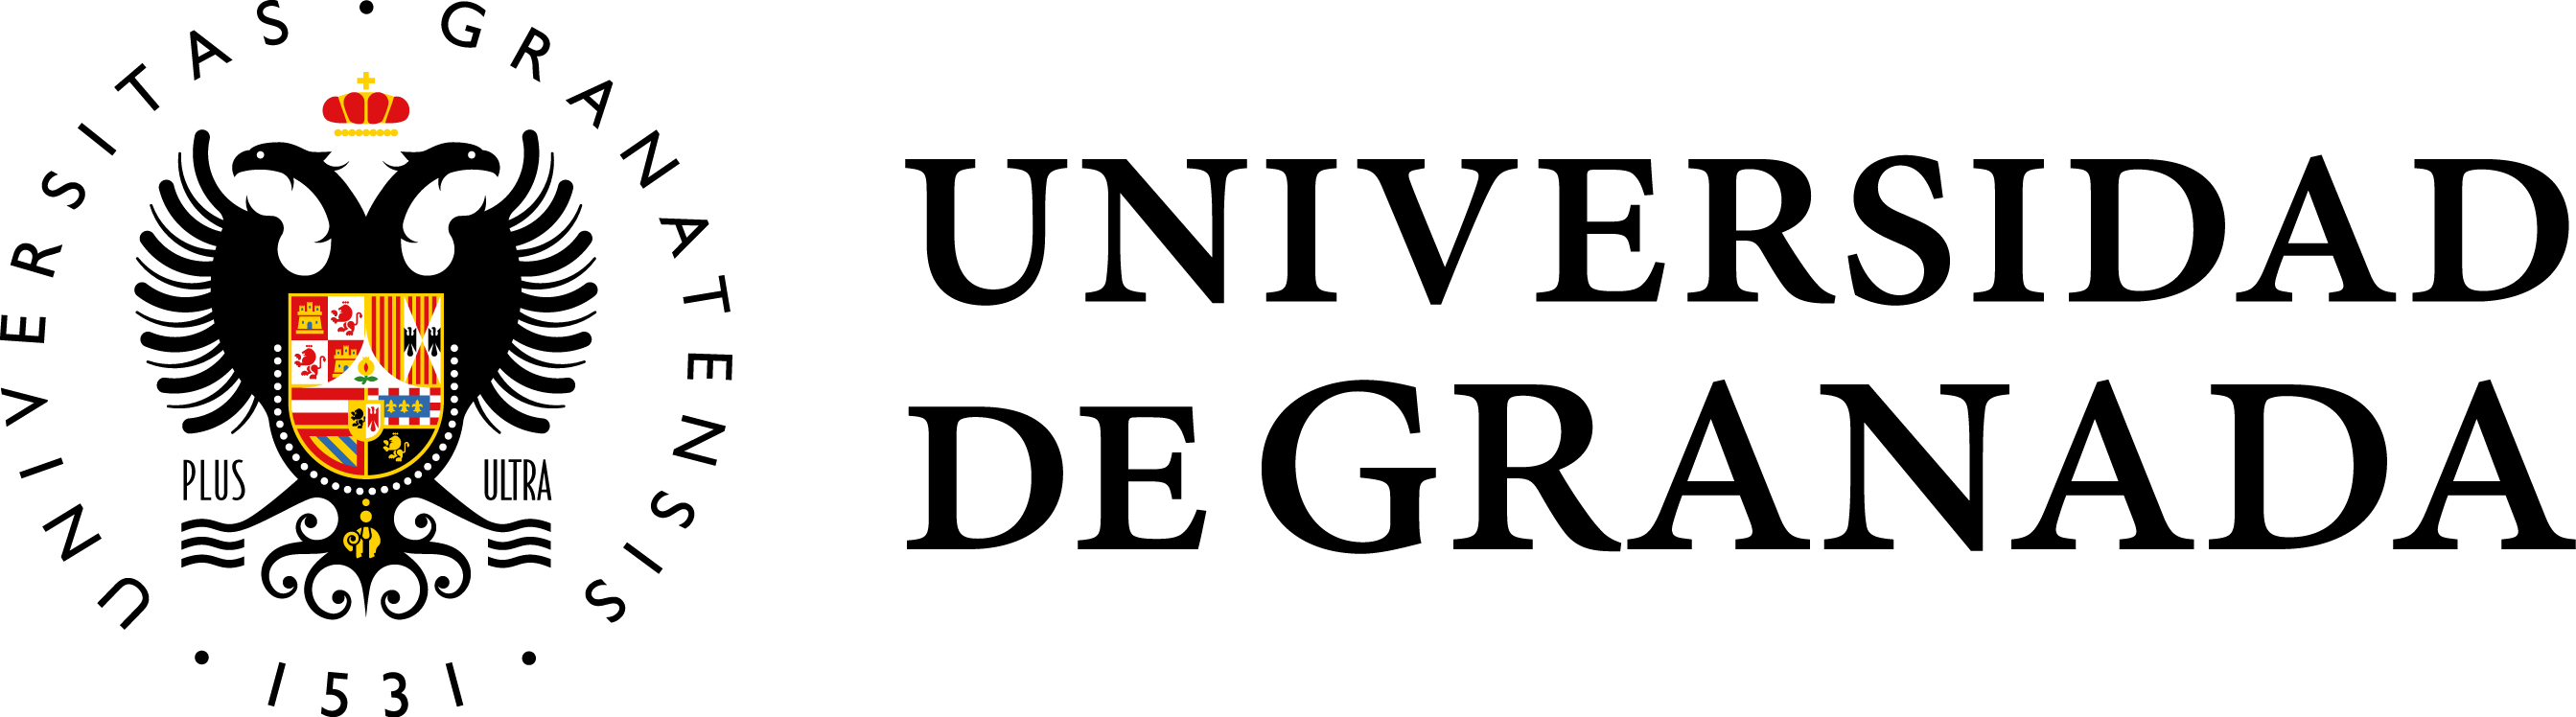
\includegraphics[width=0.25\textwidth]{../../../extraFiles/img/ugr.png} % opcional: logo
        % \vspace{1cm}
        
        % {\large \today}
    \end{center}
    
    \restoregeometry
\end{titlepage}


% ===============================
% licencia.tex
% ===============================
\section*{Licencia}

Este trabajo está licenciado bajo una 
\href{https://creativecommons.org/licenses/by-nc-nd/4.0/}{Licencia Creative Commons Reconocimiento-NoComercial-SinObraDerivada 4.0 Internacional}.

\bigskip

\textbf{Usted es libre de:}
\begin{itemize}
  \item \textbf{Compartir} — copiar y redistribuir el material en cualquier medio o formato.
\end{itemize}

\bigskip

\textbf{Bajo los siguientes términos:}
\begin{description}
  \item[\textbf{Reconocimiento}] Debe otorgar el crédito adecuado, proporcionar un enlace a la licencia e indicar si se han realizado cambios. Puede hacerlo de cualquier manera razonable, pero no de una manera que sugiera que tiene el apoyo del licenciante o lo recibe por el uso que hace.

  \item[\textbf{NoComercial}] No puede utilizar el material para fines comerciales.

  \item[\textbf{SinObraDerivada}] Si remezcla, transforma o crea a partir del material, no puede distribuir el material modificado.
\end{description}

\bigskip

\begin{center}
  \href{https://creativecommons.org/licenses/by-nc-nd/4.0/}{
\includegraphics[width=0.35\textwidth]{../../../extraFiles/img/by-nc-nd.png}}
\end{center}
  % licencia
\thispagestyle{empty} % quitar número de página en la portada
\clearpage

% --- Índice ---
\tableofcontents
% \listoffigures
\clearpage

%\listoftables
%\clearpage
%\thispagestyle{empty} % quitar número de página en la portada
%\clearpage
%
% Índice de código
%\renewcommand{\lstlistlistingname}{Índice de Código}
%\lstlistoflistings
%\clearpage
%
% Índice de ecuaciones
%\renewcommand{\listtheoremname}{Índice de Ecuaciones}
%\listoftheorems[ignoreall,show={equation}]
%\clearpage

% --- Contenido Markdown generado por Pandoc ---
\part{Teoría}

\hypertarget{introducciuxf3n}{%
\chapter{Introducción}\label{introducciuxf3n}}

Para acceder a los materiales debemos de entrar con la cuenta go.

La asignatura de Informática Gráfica tiene como objetivo principal
proporcionar los fundamentos teóricos y prácticos necesarios para el
desarrollo de aplicaciones gráficas interactivas. A lo largo del curso,
se estudian conceptos clave como la representación y modelado de
escenas, técnicas de visualización 2D y 3D, y el uso de APIs gráficas
modernas. Además, se exploran algoritmos esenciales como la
rasterización y el ray-tracing, así como su aplicación en contextos como
videojuegos, simuladores y producción de efectos visuales.

\hypertarget{aplicaciones-gruxe1ficas-interactivas-y-visualizaciuxf3n}{%
\chapter{Aplicaciones gráficas interactivas y
visualización}\label{aplicaciones-gruxe1ficas-interactivas-y-visualizaciuxf3n}}

\hypertarget{aplicaciones-gruxe1ficas-interactivas-y-proceso-de-visualizaciuxf3n-2d-y-3d}{%
\section{Aplicaciones gráficas interactivas y proceso de visualización
2D y
3D}\label{aplicaciones-gruxe1ficas-interactivas-y-proceso-de-visualizaciuxf3n-2d-y-3d}}

Un programa gráfico se define como un programa que constituye un sistema
computacional. Pueden ser interactivos o no interactivos. Los elementos
esenciales de una AG son los modelos digitales y las imágenes o vídeos
digitales que se usan.\\
Destacamos los eventos de entrada que son las acciones del usuario
mediante las cuales se envía información a la aplicación. Las
aplicaciones gráficas siempre se estructuran como un bucle de gestión de
eventos, podemos mencionar los siguientes pasos:

\begin{enumerate}
\def\labelenumi{\arabic{enumi}.}
\tightlist
\item
  Esperar al evento y recuperar datos.\\
\item
  Procesar el evento actualizando el modelo y los parámetros de
  visualización.\\
\item
  Visualizar el modelo actualizado con los nuevos parámetros.
\end{enumerate}

Las aplicaciones gráficas pueden dividirse en dos tipos:

\begin{itemize}
\tightlist
\item
  2D: los objetos se definen en planos, pueden incluir algunos 3D
  (sombras). Ejemplos de ello puede ser un diagramas de barras,
  videojuegos 2D. En este proceso de visualización se produce una imagen
  a partir de un modelo y parámetros como entradas.\\
\item
  3D: se sitúan en un espacio tridimensional, incluyendo texturas,
  materiales, fuentes de luz,\ldots{} A la vez, pueden incluir figuras
  2D. Ejemplos: videojuegos, simuladores,\ldots{} En este proceso de
  visualización se usa como entrada el modelo de escena y unos
  parámetros.

  \begin{itemize}
  \tightlist
  \item
    En el modelo de escena distinguimos dos partes:

    \begin{itemize}
    \tightlist
    \item
      Modelo geométrico: conjunto de primitivas (polígonos, planos) que
      definen los objetos a visualizar.\\
    \item
      Modelo de aspecto: parámetros que definen el aspecto de los
      objetos.\\
    \end{itemize}
  \item
    En los parámetros de visualización encontramos:

    \begin{itemize}
    \tightlist
    \item
      Cámara virtual\\
    \item
      Viewport
    \end{itemize}
  \end{itemize}
\end{itemize}

\hypertarget{rasterizaciuxf3n-versus-ray-tracing}{%
\section{Rasterización versus
ray-tracing}\label{rasterizaciuxf3n-versus-ray-tracing}}

En este apartado vamos a ver algoritmos de rasterización.

\begin{lstlisting}
1: Inicializar el color de todos los pixels al color de fondo.
2: for cada primitiva P del conjunto E do
3:     S ← conjunto de pixels de la imagen I cubiertos por P
4:     for cada pixel q de S do
5:         c ← color de la primitiva P en el pixel q
6:         Asignar el color c al pixel q en I
7:     end
8: end
\end{lstlisting}

Este pseudocódigo describe el proceso básico de rasterización, que es
una técnica utilizada para convertir primitivas geométricas (como
polígonos) en una imagen pixelada. El algoritmo recorre cada primitiva
del conjunto de entrada, determina qué píxeles de la imagen están
cubiertos por ella, calcula el color correspondiente para cada píxel y
lo asigna a la imagen final. Es un enfoque eficiente para generar
imágenes en aplicaciones gráficas interactivas.

\begin{lstlisting}
1: Inicializar el color de todos los pixels
2: for cada pixel q de la imagen I a producir do
3:     T ← subconjunto de primitivas de E que cubren q
4:     for cada primitiva P del conjunto T do
5:         c ← color de la primitiva P en el pixel q
6:         Asignar color c al pixel q en I
7:     end
8: end
\end{lstlisting}

Este pseudocódigo describe el proceso básico del algoritmo de
Ray-tracing. A diferencia de la rasterización, aquí se invierte el orden
de los bucles: se recorre cada píxel de la imagen y se determina qué
primitivas geométricas lo afectan. Luego, se calcula el color del píxel
en función de las primitivas que lo cubren. Este enfoque permite generar
imágenes con mayor realismo, aunque suele ser más costoso
computacionalmente.

En el algoritmo de Ray-tracing podemos optimizarlo de manera que la
eficiencia sea O(log n) mediante la indexación espacial.

\hypertarget{rasterizaciuxf3n}{%
\subsection{Rasterización}\label{rasterizaciuxf3n}}

Se lleva a cabo en GPUs. Es preferible para aplicaciones interactivas y
para la simulación de videojuegos, realidad virtual.

\hypertarget{ray-tracing}{%
\subsection{Ray-tracing}\label{ray-tracing}}

Respecto a la técnica de Ray-tracing:

\begin{itemize}
\tightlist
\item
  Suele ser más lento, pero consigue resultados más realistas.\\
\item
  Preferibles para elementos no interactivos. En la actualidad se usa
  para la producción de animaciones y efectos especiales.\\
\item
  Se ha usado en algunos videojuegos, pero requiere elementos
  computacionales de alto rendimiento.
\end{itemize}

\hypertarget{el-cauce-gruxe1fico-en-rasterizaciuxf3n}{%
\subsection{El cauce gráfico en
rasterización}\label{el-cauce-gruxe1fico-en-rasterizaciuxf3n}}

Cauce gráfico se define como el conjunto de etapas de cálculo para la
generación de imágenes. Las entradas se definen como primitivas. Un
vértice es un punto 2D o 3D. EL cauce escribe en el framebuffer.

Hay dos pasos importantes:

\begin{enumerate}
\def\labelenumi{\arabic{enumi}.}
\tightlist
\item
  Transformación: partiendo de las coordenadas se calculan las
  coordenadas de proyección.\\
\item
  Sombreado: cálculo del color de un pixel.\\
\item
  Hay otras como recortado de polígonos.
\end{enumerate}

Cada primitiva se sitúa en un plano imaginario (plano de visión) situado
entre el observador y la escena. La proyección puede ser perspectiva o
paralela. En la rasterización, para cada primitiva se calcula que
píxeles tienen su centro cubierto por ella. En el sombreado se usan los
atributos de la primitiva para asignar color al píxel.

\hypertarget{etapas-del-cauce-gruxe1fico}{%
\subsubsection{Etapas del cauce
gráfico}\label{etapas-del-cauce-gruxe1fico}}

\begin{enumerate}
\def\labelenumi{\arabic{enumi}.}
\tightlist
\item
  Procesado de vértices

  \begin{enumerate}
  \def\labelenumii{\arabic{enumii}.}
  \tightlist
  \item
    Transformación: los vértices de cada primitiva se transforman para
    encontrar su proyección en el plano.\\
  \item
    Teselación y nivel de detalle: transformaciones avanzadas.\\
  \end{enumerate}
\item
  Post-procesado de vértices y montaje de primitivas\\
\item
  Rasterización\\
\item
  Sombreado
\end{enumerate}

\incluirimagen[scale=0.7]{media/cauce1.png}{Esquema del cauce}

\hypertarget{apis-y-motores-gruxe1ficos}{%
\section{APIs y motores gráficos}\label{apis-y-motores-gruxe1ficos}}

\hypertarget{apis-para-rasterizaciuxf3n-ray-tracing-y-gpgpu}{%
\subsection{APIs para Rasterización, Ray-tracing y
GPGPU}\label{apis-para-rasterizaciuxf3n-ray-tracing-y-gpgpu}}

APIs de rasterización: conjunto de funciones para visualización 2D/3D,
clases, interfaces. Son definidas sin ánimo de lucro, se puede dejar
compilado en código intermedio.

APIs gráficas: estas proporcionan portabilidad y acceso simultáneo. La
escritura en el framebuffer sigue siendo lenta, esto se soluciona usando
GPU y enviando información de alto nivel a través del bus del sistema.

Como ejemplos podemos mencionar OpenGL, Vulkan, Metal, \ldots{}

Las APIs modernas son más eficientes aunque tienen ciertas desventajas
como más complejidad y menos portabilidad.

\hypertarget{motores-gruxe1ficos}{%
\subsection{Motores gráficos}\label{motores-gruxe1ficos}}

\begin{definicion}
Conjunto de herramientas software que facilita la creación de aplicaciones gráficas interactivas, como videojuegos, aunque se usa en la simulación, realidad virtual, ... Incluye motor de renderización y otras muchas herramientas. Permite crear aplicaciones gráficas portables y más. Algunos son de código abierto. Estos motores gráficos usan APIs gráficas como OpenGL, ...
\end{definicion}

El \emph{grafo de escena} o \emph{jerarquía} es una estructura de datos
que modela las relaciones jerárquicas entre los objetos.

El término \emph{visual scripting} se define como la posibilidad de
programar aspectos de la aplicación gráfica creando un grafo que
codifica un \textbf{diagrama de flujo de datos}.

Los motores gráficos permiten programar partes usando lenguajes
tradicionales como c++, entre otros.

\begin{definicion}
Un shader en un motor gráfico es un programa pequeño que se ejecuta en la GPU (tarjeta gráfica) y que define cómo deben procesarse y representarse los píxeles, vértices o fragmentos de una escena 3D en pantalla.
\end{definicion}

Se pueden programar los shaders mediante visual scripting y lenguajes de
shading.

Principales motores gráficos: Unreal Engine, Unity, CryEngine y de
fuentes abiertas: Godot, Armory3D.

\hypertarget{el-engine-godot.-mallas.}{%
\chapter{El engine Godot. Mallas.}\label{el-engine-godot.-mallas.}}

\hypertarget{introducciuxf3n-a-godot}{%
\section{Introducción a Godot}\label{introducciuxf3n-a-godot}}

\underline{Funcionalidad y características de Godot}

Godot es un IDE (entorno integrado de desarrollo) que permite
desarrollar aplicaciones gráficas interactivas en 2D y 3D, como
videojuegos, simulaciones y visualizaciones. Además, facilita la
ejecución, depuración y generación de archivos ejecutables
independientes para diversas plataformas.

Entre sus características principales destacan:

\begin{itemize}
\tightlist
\item
  \textbf{Código abierto}: completamente gratuito y con una comunidad
  activa.
\item
  \textbf{Multiplataforma}: el IDE puede ejecutarse en Linux, Windows,
  macOS e incluso en navegadores web (con ciertas limitaciones).
\item
  \textbf{Generación de aplicaciones multiplataforma}: permite crear
  aplicaciones nativas para Windows, macOS, Linux, Android, iOS y Web.
\end{itemize}

\textbf{Elementos de Godot}

\begin{itemize}
\tightlist
\item
  \textbf{Editor}: herramienta tipo IDE que organiza recursos, diseña
  escenas, programa scripts y permite ejecutar y depurar aplicaciones.
\item
  \textbf{Proyecto}: conjunto de escenas, nodos, scripts y recursos
  asociados a una aplicación.
\item
  \textbf{Escenas}: estructuras jerárquicas (árboles de nodos) que
  representan los elementos de la aplicación.
\item
  \textbf{Nodos}: componentes de las escenas, cada uno perteneciente a
  una clase específica de Godot.
\item
  \textbf{Scripts}: código que define el comportamiento de nodos y
  escenas, utilizando GDScript (similar a Python), C\#, o el lenguaje
  visual de Godot.
\item
  \textbf{Recursos}: archivos como imágenes, audios, videos y modelos 3D
  utilizados en el desarrollo de la aplicación.
\end{itemize}

\hypertarget{el-lenguaje-de-programaciuxf3n-gdscript}{%
\subsection{El lenguaje de programación
GDScript}\label{el-lenguaje-de-programaciuxf3n-gdscript}}

GDScript es un lenguaje de programación interpretado, de alto nivel y
orientado a objetos.

\begin{itemize}
\tightlist
\item
  Tiene una sintaxis similar a python. Usando la indentación de manera
  similar.
\item
  Las variables no tienen porque tener siempre asociado un tipo.
  \footnote{En las transparencias está mal. Página 7/84.}
\item
  Es orientado a objetos.
\item
  Gestión automática de memoria mediante conteo de referencias.
\item
  Especiamente diseñado para Godot.
\end{itemize}

\begin{lstlisting}
extends Node3D # obligatorio: indica la clase base

class_name MiNodo # opcional: si no está es una clase anónima

var velocidad : float = 100.0 # variable de instancia (tipo opc.)

func v_cuadrado() -> float : # método que devuelve un float
 return velocidad * velocidad # devuelve la velocidad al cuadrado

func _init(): # constructor, puede tener parámetros
 pass # 'pass' indica que está vacío

func _ready(): # método de nodo listo
 print("Nodo listo") # imprime en la consola o terminal

func _process( delta: float ): # método de proceso por frame
 position.x += velocidad * delta # usa 'position' de Node2D
\end{lstlisting}

Extensión .gd, siempre definen una clase, aunque puede ser anónima, que
siempre hereda de otra.

\textbf{Tipos básicos y contenedores en GDScript}

\begin{itemize}
\item \textbf{bool}: valores lógicos (true o false).
\item \textbf{int}: enteros de 64 bits.
\item \textbf{float}: números reales de doble precisión (64 bits).
\item \textbf{String}: cadenas de caracteres en Unicode.
\end{itemize}

\begin{itemize}
\item \textbf{Vector2, Vector3, Vector4}: tuplas con 2, 3 o 4 elementos flotantes (32 bits).
\item \textbf{Vector2i, Vector3i, Vector4i}: tuplas con 2, 3 o 4 elementos enteros.
\item \textbf{Transform2D, Transform3D}: matrices de transformación en 2D o 3D.
\end{itemize}

\begin{itemize}
\item \textbf{Color}: colores en formato RGBA.
\end{itemize}

\begin{itemize}
\item \textbf{Array}: dinámico, puede contener elementos de cualquier tipo (Variant).
\item \textbf{Array[T]}: homogéneo, todos los elementos son del tipo T.\footnote{Debemos de tener cuidado al eliminar y añadir elementos, para garantizar la continuidad de los elementos se recomienda copiarlos completamente en otra array.}
\item \textbf{Arrays empaquetados}: homogéneos y contiguos en memoria, ideales para GPU:
  \begin{itemize}
  \item \textbf{PackedByteArray, PackedInt32Array, PackedInt64Array}: bytes o enteros.
  \item \textbf{PackedFloat32Array, PackedFloat64Array}: flotantes de simple o doble precisión.
  \item \textbf{PackedVector2Array, PackedVector3Array, PackedVector4Array}: vectores.
  \item \textbf{PackedColorArray}: colores.
  \end{itemize}
\end{itemize}

\emph{Permite tipos estáticos y dinámicos.}

\begin{lstlisting}
var x : float = 10.0 # tipo 'float' (explícito) 
  # tipo explícito, no puede cambiar de tipo a lo largo de su vida

var y := 20 # tipo 'int' (es el tipo de la expresión '20').
  # implícito inferido, se infiere a partir de la expresión inicial

var z = 30.0 # sin tipo (inicialmente 'float', pero puede cambiar)
  # sin tipo, este puede cambiar a lo largo de su vida
\end{lstlisting}

\underline{Ventajas del Tipado Estático}

El tipado estático ofrece múltiples beneficios:

\begin{itemize}
\tightlist
\item
  \textbf{Detección temprana de errores}: Identifica errores en tiempo
  de desarrollo, reduciendo el tiempo de depuración y evitando problemas
  en producción.
\item
  \textbf{Mejor rendimiento}: Optimiza la ejecución al eliminar la
  necesidad de verificar tipos en tiempo de ejecución.
\item
  \textbf{Legibilidad y comprensión}: Facilita la lectura del código al
  hacer explícitos los tipos de las variables.
\item
  \textbf{Expresividad}: Los tipos implícitos permiten un código más
  conciso, aunque pueden afectar la legibilidad en ciertos casos.
\end{itemize}

\hypertarget{jerarquuxeda-de-clases-de-godot}{%
\subsection{Jerarquía de clases de
Godot}\label{jerarquuxeda-de-clases-de-godot}}

Las clases de Godot están organizadas en una jerarquía de herencia,
donde la clase Object es la raíz. Todas las demás clases heredan directa
o indirectamente de ella. Algunas clases derivadas importantes son:

\begin{itemize}
\tightlist
\item
  Node: base para nodos de escenas, como visualización 2D/3D, controles,
  cámaras, luces, materiales, y más.
\item
  Viewport: define una zona rectangular donde se renderiza una escena.
  Cada proyecto tiene un Viewport por defecto.
\item
  MainLoop: clase abstracta para implementar el bucle principal de la
  aplicación. SceneTree es su implementación por defecto.
\end{itemize}

Otras clases derivadas incluyen:

\begin{itemize}
\tightlist
\item
  RefCounted: gestiona objetos en memoria dinámica con cuenta de
  referencias.

  \begin{itemize}
  \tightlist
  \item
    Resource: base para recursos de Godot, como:

    \begin{itemize}
    \tightlist
    \item
      Mesh: para mallas 2D/3D. Las mallas ocupan demasiado espacio por
      lo que duplicarlo es demasiado costoso.
    \item
      Material: para definir la apariencia visual de objetos.
    \item
      Image, Texture: para imágenes y texturas.
    \item
      Shader: para programas que se ejecutan en la GPU.
    \end{itemize}
  \end{itemize}
\end{itemize}

Godot incluye diversos tipos de nodos organizados jerárquicamente. Entre
los nodos principales destacan:

\begin{itemize}
\tightlist
\item
  \textbf{CanvasItem}: base para elementos visuales en 2D, con subclases
  como:

  \begin{itemize}
  \tightlist
  \item
    Control: interfaz de usuario (botones, menús, etc.).
  \item
    Node2D: objetos 2D en escenas 2D.
  \end{itemize}
\item
  \textbf{Node3D}: base para objetos 3D, con subclases como:

  \begin{itemize}
  \tightlist
  \item
    VisualInstance3D: mallas y luces.
  \item
    Camera3D: cámaras en escenas 3D.
  \end{itemize}
\end{itemize}

En cuanto a mallas, la clase \textbf{Mesh} es la base para representar
primitivas geométricas en 2D/3D. Sus subclases incluyen:

\begin{itemize}
\tightlist
\item
  ArrayMesh: definida por programador, permanece en GPU.
\item
  ImmediateMesh: enviada a GPU en cada frame.
\item
  PrimitiveMesh: primitivas predefinidas como BoxMesh, SphereMesh, etc.
\end{itemize}

Nodos específicos para 2D y 3D permiten instanciar mallas, cámaras y
luces, como MeshInstance2D, Sprite2D, MeshInstance3D, y Light3D
(DirectionalLight3D, OmniLight3D, SpotLight3D). Estos nodos facilitan la
creación y manipulación de escenas gráficas.

Las mallas pueden tener referencias a muchas mallas o solo una
referencia a un mesh (lo que está en la GPU).

Godot define varias clases para representar tuplas de valores, entre
ellas tenemos Vector2, Vector3, Vector 4 (para float), con el sufijo i
(para int), color para colores RGBA, Rect2 para rectángulos 2D.

La clase abstracta MainLoop define métodos que permite configurar el
comportamiento de cualquier aplicación creada con Godot. Los métodos son
\textbf{\_initialize}, \textbf{\_process} y \textbf{\_finalize}. Cuando
se ejecuta se dan estos pasos:

\begin{enumerate}
\def\labelenumi{\arabic{enumi}.}
\tightlist
\item
  Se crea una instancia de la clase derivada de MainLoop (SceenTree),
  creando el árbol de inicio, dándole los valores por defecto que hay en
  el editor.
\item
  Se invoca al método \textbf{\_initialize}
\item
  Mientras no se termine la aplicación:

  \begin{enumerate}
  \def\labelenumii{\arabic{enumii}.}
  \tightlist
  \item
    Se invoca a \textbf{\_process} par actualizar el estado de los
    objetos de la aplicación.
  \item
    Si es necesario, se hace una espera hasta que sea el momento del
    siguiente frame.
  \end{enumerate}
\item
  Se invoca al método \textbf{\_finalize}.
\end{enumerate}

\underline{Clase SceneTree}

\begin{itemize}
\tightlist
\item
  Implementación concreta de MainLoop.
\item
  Creación del árbol.
\item
  Gestión de nodos.
\item
  Actualización de frames.
\item
  Cálculos asociados.
\item
  Entrada de usuario.
\item
  Ejecución de scripts.
\item
  Terminación y liberación de recursos.
\end{itemize}

Se puede diseñar el árbol de escena

\begin{itemize}
\tightlist
\item
  Antes de ejecutar. Para ello debe de crear un nodo y asignarle un
  script que redefine varios métodos de la calse Node. Por otro lado, se
  puede crear un nodo de clase definido por el usuario, que herede de
  Node. Esa clase pude tener métodos específicos.
\item
  En tiempo de ejecución. Creando un nodo h con el método new de su
  clase y añadiéndolo al árbol como un hijo de un nodo p existente.
\end{itemize}

\begin{lstlisting}
# Añadir nodos hijos a una malla
var h:= ArrayMesh.new()
p.add_child(h)
\end{lstlisting}

\underline{Redefinición de métodos}

El comportamiento de un nodo puede adaptarse redefiniendo métodos de
Node u Object que se invocan por SceneTree en determinados momentos
durante la ejecución:

\begin{itemize}
\tightlist
\item
  \textbf{\_init}: Constructor del nodo (método de Object), se invoca al
  crear un nodo para inicializar sus variables de instancia. Puede tener
  parámetros.
\item
  \textbf{\_enter\_tree}: Se invoca al añadir un nodo al árbol, cuando
  su padre se ha añadido, pero antes de añadir sus hijos.
\item
  \textbf{\_ready}: Se invoca al añadir el nodo, después de
  \textbf{\_enter\_tree}, cuando ya se han añadido los nodos hijos.
\item
  \textbf{\_process(delta)}: Se invoca antes de cada frame para
  actualizar el estado del nodo. El parámetro delta indica el tiempo (en
  segundos) transcurrido desde el último frame.
\item
  \textbf{\_input(event)}: Invocado cuando se produce un evento de
  entrada (teclado, ratón, etc.). El parámetro event lleva información
  del evento.
\end{itemize}

\hypertarget{mallas-en-godot}{%
\section{Mallas en Godot}\label{mallas-en-godot}}

Cada primitiva o conjunto de primitivas se especifica mediante una
secuencia ordenada de vértices. Un vértice es un espacio afín en 3D,
puede tener asociado otros valores como colores, \ldots{}

Existen 3 tipos de primitivas: puntos segmentos y triángulos.

A cada forma de codificar primitivas en una secuencia se le llama un
tipo de primitivas, en GDScript se definen diversas constantes para eso,
del tipo enumerado PrimitiveType, en la clase Mesh.

\begin{longtable}[]{@{}
  >{\raggedright\arraybackslash}p{(\columnwidth - 2\tabcolsep) * \real{0.2832}}
  >{\raggedright\arraybackslash}p{(\columnwidth - 2\tabcolsep) * \real{0.7168}}@{}}
\toprule\noalign{}
\begin{minipage}[b]{\linewidth}\raggedright
\textbf{Tipo de primitiva}
\end{minipage} & \begin{minipage}[b]{\linewidth}\raggedright
\textbf{Descripción}
\end{minipage} \\
\midrule\noalign{}
\endhead
\bottomrule\noalign{}
\endlastfoot
Mesh.PRIMITIVE\_POINTS & n puntos aislados (n arbitrario) \\
Mesh.PRIMITIVE\_LINES & n/2 segmentos independientes (n debe ser par) \\
Mesh.PRIMITIVE\_LINE\_STRIP & n - 1 segmentos formando una polilínea
abierta (n debe ser mayor o igual a 2) \\
Mesh.PRIMITIVE\_TRIANGLES & n/3 triángulos (n debe ser múltiplo de 3),
siempre debe de estar relleno de algo, una textura, \ldots{} \\
Mesh.PRIMITIVE\_TRIANGLE\_STRIP & n - 2 triángulos compartiendo aristas
(tira de triángulos), (n debe ser mayor o igual a 3) \\
\end{longtable}

Una secuenci a de coordenadas \((v_0, v_1, v_2, \ldots, v_{n-1})\)
pueden formar puntos, segmentos o polilíneas abiertas.

\incluirimagen{media/ejemplo1.png}{Con n=6}

Cada primitiva de tipo triángulo tiene dos caras:

\begin{itemize}
\tightlist
\item
  Delantera: si sus vértices se visualizan en pantalla en el sentido
  contrario de las agujas del reloj.
\item
  Trasera: sentido de las agujas del reloj.
\end{itemize}

Godot puede ser configurado para visualizar solo las delanteras, las
traseras o ambas, esto se conoce como hacer \emph{cribado de caras}. Por
defecto, solo visualiza las delanteras.

\dosimagenes{media/primitivas.png}{Esquema}{media/primitivas1.png}{Necesidad de repetir coordenadas}{pri1}{pr22}

En la figura \label{fig:pr1} podemos ver los puntos en las coordendas y
un esquema de las aristas de los triángulos que se formarían.

En la figura \label{fig:pr22} es un ejemplo de cuando necesitamos
repetir coordenadas, para ver 7 triángulos como es ese caso. Usando
\emph{GL\_TRIANGLES}, necesitamos esta secuencia de vértices:

\begin{align*}
V_0, V_2, V_1, & \quad V_1, V_2, V_3, & \quad V_1, V_3, V_4, & \quad V_2, V_5, V_3, & \quad V_3, V_5, V_6, & \quad V_3, V_6, V_7, & \quad V_3, V_7, V_4
\end{align*}

Supone emplear más memoria y tiempo para visualizar el escenario. Tiene
21 coordenadas de vértices, pero solo 8 son distintos.

\underline{Secuencias Indexadas}

Para solucionar el problema anterior relacionado con la memoria, las
APIs y engines, permiten especificar una secuencia de vértices a partir
de una secuencia de vértices únicos.

\begin{itemize}
\item Se parte de una secuencia $V_n$ de $n$ coordenadas arbitrarias de vértices $V_n = \{v_0, v_1, ..., v_{n-1}\}$.
\item Se usa una secuencia $I_m$ de $m$ índices $I_m = \{i_0, i_1, ..., i_{m-1}\}$ donde cada valor $i_j$ es un entero entre $0$ y $n-1$ (ambos incluidos). Puede haber valores repetidos.
\item La secuencia de vértices $V_n$ y la de índices determinan otra secuencia $S_m$ de $m$ vértices:
\[
S_m = \{v_{i_0}, v_{i_1}, ..., v_{i_{m-1}}\}
\]
que tiene las mismas coordenadas de vértices de $V_n$ pero en el orden especificado por los índices en $I_m$.
\end{itemize}

En el ejemplo de la figura \label{fig:pr2} usaríamos una lista de
índices (cada tres forman un triángulo).

\[
V_8 = \{v_0, v_1, v_2, v_3, v_4, v_5, v_6, v_7\}
\] \[
I_{21} = \{0, 2, 1, 1, 2, 3, 1, 3, 4, 2, 5, 3, 3, 5, 6, 3, 6, 7, 3, 7, 4\}
\]

\nota{Nota}{Debemos de tener en cuenta que en la primera tabla se referencia una sola vez, mientras que en la tabla de triángulos se referencia dos veces.}

\hypertarget{atributos-de-vuxe9rtices}{%
\subsection{Atributos de vértices}\label{atributos-de-vuxe9rtices}}

Las coordenadas de su posición se considera una atributo de vértices,
siendo este imprescindible. Además, hay otros como el color, la normal
\footnote{Vector unitario con tres coordenadas reales que determina la orientación de la superficie de un obeto en el punto donde está el vértice.}
y las coordenadas de textura
\footnote{Típicamente un par de valores reales, que se usan para determinar que punto de textura se fija al vértice.}.

\underline{Colores de vértices}

Podemos añadir en los triángulos tres colores codificados con una terna
RGB, de manera que se produciría una interpolación de los colores (para
calcular cada pixel), o bien, una cuádrupla añadiendole transparencia.

\underline{Normales}

A cada vértice se le puede asociar un vector de 3 componentes
\((x,y,z)\), su vector normal, que determina la orientación de la
superficie en ese vértice para hacer el sombreado y la iuminación.

\underline{Coordenadas de texturas}

Podemos asociar a cada vértice una dupla \((s,t)\), que corresponden a
sus coordenadas de textura, típicamente en \([0,1]^2\).

\underline{Definición de valores de los atributos}

En Godot, cada vértice tiene asociados varios atributos, como posición,
color, normal y coordenadas de textura, entre otros como hemos visto. La
utilización de estos atributos depende de la configuración del cauce
gráfico. Por ejemplo:

\begin{itemize}
\tightlist
\item
  Si un objeto no tiene textura, las coordenadas de textura no se
  usarán.
\item
  Si la iluminación está desactivada, las normales no serán utilizadas.
\end{itemize}

Es posible definir un único valor de un atributo para todos los vértices
de una primitiva o especificar valores individuales para cada vértice.
Durante la rasterización, los valores de los atributos en cada píxel se
calculan mediante interpolación, permitiendo una representación visual
más precisa y detallada.

\hypertarget{modos-de-envuxedos-de-datos-a-la-gpu}{%
\subsection{Modos de envíos de datos a la
GPU}\label{modos-de-envuxedos-de-datos-a-la-gpu}}

Las GPUs modernas estan diseñadas para visualizar secuencias de vértices
y atributos almacenados en la memoria de la GPU. Esto se debe que el
acceso a su propia memoria es más rápido que a la del sistema. Pero, el
origen de los datos estará en el sistema, es decir, siempre quedan
inicialmente en la CPU. Es necesario realizar un envío de datos desde la
CPU a la GPU para esto.

Para ello se puede realizar de dos formas:

\begin{itemize}
\tightlist
\item
  Modo inmediato: cada vez que queremos visualizar un frame, se envían
  atributos e índices a la GPU por el bus del sistema. Este modo es muy
  ineficiente en tiempo, ya que el ancho de banda del bus del sistema es
  limitado.
\item
  Modo diferido: los datos de la secuencia de vértices se envían a la
  GPU una vez, como parte de la inicialización de la aplicación. Emplea
  menos tiempo por cuadro que el anterior, ya que la transferencia de
  datos se hace menos veces, suele ser una vez.
\end{itemize}

Por defecto, se suele usar el envío en modo diferido, debido a su mayor
eficiencia. En algunos casos, es conveniente usar el de envío inmediato,
para ello es aconsejable que se den estas dos condiciones:

\begin{itemize}
\tightlist
\item
  Secuencia de vértices y atributos es actualizada por la aplicación con
  mucha frecuencia.
\item
  La secuencia es pequeña.
\end{itemize}

El envio previo a cada frame de los datos actualizables es realizable ya
que no penaliza mucho el tiempo debido a que la secuencia de vértices no
ocupa mucho espacio.

En mallas grandes se usa el envío diferido.

Godot usa normalmente el envío diferido, para los nodos que contienen
mallas en 2D y 3D. Se puede usar el envío en modo inmediato usando nodos
específicos para ello.

\hypertarget{representaciuxf3n-de-mallas-en-godot}{%
\subsection{Representación de mallas en
Godot}\label{representaciuxf3n-de-mallas-en-godot}}

Las APIs y engines suelen ofrecer dos formas de almacenar arrays de
posiciones de vértices y sus atributos: - Array de estructuras (AOS
Array of Structures): usa un array o un vector donde cada entrada tiene
las coordenadas de un vértice y todos sus atributos. - Estructura de
arrays (SOA Structure of Arrays): usa una estructura con varios punteros
a arrays de número de elementos. Uno de ellos contiene las coordenadsa y
los otros contienen cada uno una tabla de atributos.

Los índices siempre están contiguos en su propio array. En Godot se usa
la opción SOA.

En este lenguaje que venimos viendo se contemplan diversos tipos de
datos para guardar tuplas con valores reales:

\begin{itemize}
\tightlist
\item
  Vector2: tupla de dos reales.
\item
  Vector3: tupla de tres reales.
\item
  Color: tupla de 4 reales.
\end{itemize}

Se suele asociar un valor entero a cada atributo de vértice. Se define
en este lenguaje el tipo de enumerado ArrayType en la clase Mesh.

\begin{table}[H]
\centering
\begin{tabular}{|l|c|l|}
\hline
\textbf{Identificador}         & \textbf{Valor} & \textbf{Significado}                                   \\ \hline
Mesh.ARRAY\_VERTEX             & 0              & Coordenadas de posición (obligatorias)                \\ \hline
Mesh.ARRAY\_NORMAL             & 1              & Vector normal                                         \\ \hline
Mesh.ARRAY\_TANGENT            & 2              & Vector tangente                                       \\ \hline
Mesh.ARRAY\_COLOR              & 3              & Color RGB                                            \\ \hline
Mesh.ARRAY\_TEX\_UV            & 4              & Coordenadas de textura                               \\ \hline
Mesh.ARRAY\_TEX\_UV2           & 5              & Segundas coordenadas de textura                     \\ \hline
Mesh.ARRAY\_CUSTOM0--3         & 6 -- 9         & Atributos definidos por el usuario                  \\ \hline
\end{tabular}
\caption{Atributos de vértices en Godot}
\end{table}

Las tablas de atributos de vértices se pueden codificar en arrays
empaquetados.

\begin{table}[H]
\centering
\begin{tabular}{|l|l|l|}
\hline
\textbf{Atributo}         & \textbf{Clase array}         & \textbf{Tipo elem.} \\ \hline
Posiciones 2D             & PackedVector2Array          & Vector2             \\ \hline
Posiciones 3D             & PackedVector3Array          & Vector3             \\ \hline
Colores                   & PackedColorArray            & Color               \\ \hline
Normales                  & PackedVector3Array          & Vector3             \\ \hline
Coords. textura           & PackedVector2Array          & Vector2             \\ \hline
\end{tabular}
\caption{Atributos de vértices y sus arrays empaquetados en Godot}
\end{table}

\subsubsection*{Clases de Mallas en Godot}

\begin{itemize}
\item ArrayMesh: derivada de Mesh, contiene una malla que se visualizará en modo diferido.
\item InmediateMesh: derivada de Mesh, contiene una malla que se visualizará en modo inmediato. 
\item SurfaceTool: derivada de RefCounted.
\item MeshInstance2D: derivada de Node2D, permite instanciar una malla en 2D.
\item MeshInstance3D: derivada de Node3D, permite instanciar una malla en 3D.
\end{itemize}

\underline{Ahora vamos a ver varios ejemplos con mallas 2D y 3D.}

\hypertarget{mallas-en-2d}{%
\subsection{Mallas en 2D}\label{mallas-en-2d}}

\includecode[gdstyle]{code/sesion2/mallas2D/mallanoindentada.gd}{Malla sin indentación}
\includecode[gdstyle]{code/sesion2/mallas2D/mallaconcoloresdevertices.gd}{Malla con colores de vértices}
\includecode[gdstyle]{code/sesion2/mallas2D/cargatexturas.gd}{Carga de texturas en mallas 2D}
\includecode[gdstyle]{code/sesion2/mallas2D/envioinmediato.gd}{Envío inmediato de mallas 2D}
\includecode[gdstyle]{code/sesion2/mallas2D/malla2dcontexturas.gd}{Malla 2D con texturas}

\hypertarget{mallas-en-3d}{%
\subsection{Mallas en 3D}\label{mallas-en-3d}}

\includecode[gdstyle]{code/sesion2/mallas3D/mallaindexada3d.gd}{Malla indexada en 3D}
\includecode[gdstyle]{code/sesion2/mallas3D/materialconcoloresdevertices.gd}{Material con colores de vértices en 3D}
\includecode[gdstyle]{code/sesion2/mallas3D/materialconcolordeplano.gd}{Material con color de plano en 3D}
\includecode[gdstyle]{code/sesion2/mallas3D/tablas.gd}{Tablas en mallas 3D}

\part{Prácticas}

\hypertarget{introducciuxf3n-1}{%
\chapter{Introducción}\label{introducciuxf3n-1}}

Las prácticas de la asignatura se llevaran acabo con \emph{Godot}.

Un motor de juego es una herramienta compleja y difícil de presentar en
pocas palabras. Aquí hay una rápida sinopsis, que eres libre de
reutilizar si necesitas una breve reseña sobre Godot Engine:

Godot Engine es un motor de videojuegos repleto de características,
multiplataforma para crear juegos 2D y 3D por medio de una interfaz
unificada. Provee un conjunto exhaustivo de herramientas comunes, para
que los usuarios puedan enfocarse en crear juegos sin tener que
reinventar la rueda. Los juegos pueden exportarse en un sólo clic a
numerosas plataformas, incluyendo las principales plataformas de
escritorio (Linux, macOS, Windows), plataformas móviles (Android, iOS),
así como plataformas y consolas basadas en la web.

Godot es completamente gratis y de código abierto bajo la permisiva
licencia MIT (Licencia del Instituto Tecnológico de Massachusetts). Sin
condiciones, sin regalías, nada. Los juegos de los usuarios son suyos,
hasta la última línea de código del motor. El desarrollo de Godot es
totalmente independiente y dirigido por la comunidad, lo que permite a
los usuarios ayudar a dar forma a su motor para que coincida con sus
expectativas. Está respaldado por la Godot Foundation (Fundación Godot)
sin fines de lucro.\footnote{\url{https://docs.godotengine.org/es/4.x/}}

Para la \emph{descarga} de Godot debemos de hacerlo mediante el enlace
de la web oficial \footnote{\url{https://godotengine.org/es/}}.

\nota{Nota}{El equipo de Godot no puede proporcionar una exportación de consola de código abierto debido a los términos de licencia impuestos por los fabricantes de consolas. Independientemente del motor que use, lanzar juegos en consolas siempre es mucho trabajo. Puedes leer más sobre eso en el Soporte de consolas en Godot.}

Se recomienda encarecidamente leer el \emph{started} de Godot
\footnote{\url{https://docs.godotengine.org/es/4.x/getting_started}}.

\hypertarget{aprendiendo-a-programar-con-godot}{%
\section{Aprendiendo a programar con
Godot}\label{aprendiendo-a-programar-con-godot}}

En Godot, es posible escribir código utilizando los lenguajes de
programación GDScript y C\#. Para aprender los lenguajes relacionados,
podemos realizar el curso de manera interactiva que nos
ofrecen.\footnote{\url{https://gdquest.github.io/learn-gdscript}}

Ejemplo de GDScript comparando con otros lenguajes que ya conocemos

\begin{lstlisting}
# GDScript
func take_damage(amount):
    health -= amount
    if health < 0:
        die()
\end{lstlisting}

\begin{lstlisting}[language=Python]
# Python
def take_damage(amount):
    health -= amount
    if health < 0:
        die()
\end{lstlisting}

\begin{lstlisting}
# Javascript
function takeDamage(amount) {
    health -= amount;
    if (health < 0) {
        die();
    }
}
\end{lstlisting}

Además, en el curso se nos ofrece la posibilidad de ir practicando como
vemos en la figura \ref{fig:media/course1.png}.

\incluirimagen{media/course1.png}{Imagen de práctica}

\hypertarget{conceptos-clave-de-godot}{%
\section{Conceptos clave de Godot}\label{conceptos-clave-de-godot}}

Todos los motores de videojuegos giran alrededor de abstracciones que
usas para crear tus aplicaciones. En Godot, un juego es un árbol de
nodos agrupados en escenas. Los nodos pueden comunicarse entre sí
mediante señales.

\begin{itemize}
    \item \textbf{Escenas:} En Godot, puedes dividir tu juego en escenas reutilizables, como personajes, niveles o menús. Estas escenas pueden combinarse y anidarse para formar estructuras más complejas.

    \item \textbf{Nodos:} Las escenas están compuestas por nodos, que son los bloques de construcción básicos de tu juego. Godot ofrece una amplia biblioteca de nodos base que puedes combinar y extender.

    \item \textbf{El árbol de escenas:} El árbol de escenas organiza todas las escenas y nodos de tu juego. Representa la jerarquía y estructura general de tu proyecto.

    \item \textbf{Señales:} Los nodos emiten señales para comunicar eventos, como colisiones o interacciones. Esto permite una comunicación flexible entre nodos sin acoplamiento directo.

    \item \textbf{Sumario:} Los nodos, escenas, el árbol de escenas y las señales son los conceptos fundamentales de Godot. Estos elementos te permitirán estructurar y desarrollar tus juegos de manera eficiente.
\end{itemize}

\hypertarget{pruxe1ctica-1}{%
\chapter{Práctica 1}\label{pruxe1ctica-1}}

\dosimagenes{media/p1-diferentes-tonalidades.png}{Diferentes tonalidades}{media/p1-piramide.png}{Pirámide}{tonalidades}{piramide}

\incluirimagen{media/p1-final.png}{Resultado final}

\begin{thebibliography}{99}

  \bibitem{Referencia1}
  Ismael Sallami Moreno, \textbf{Estudiante del Doble Grado en Ingeniería Informática + ADE}, Universidad de Granada, 2025.
  
  \bibitem{DiapositivasAsignatura}
  Universidad de Granada, \emph{Diapositivas de la asignatura}, Curso 2025/2026.

  % \bibitem{Referencia2}
  % Autor Apellido, \emph{Título del libro o artículo}, Editorial o Revista, Año.
  
  % \bibitem{Referencia3}
  % Nombre Autor, \emph{Título del documento}, Conferencia/URL, Año.
  
  \end{thebibliography}
  

\end{document}
